\documentclass[conference]{IEEEtran}
\IEEEoverridecommandlockouts
% The preceding line is only needed to identify funding in the first footnote. If that is unneeded, please comment it out.
\usepackage{cite}
\usepackage{amsmath,amssymb,amsfonts}
\usepackage{algorithmic}
\usepackage{graphicx}
\usepackage{textcomp}
\usepackage{xcolor}
\newtheorem{remark}{Tvrdnja}[section]
\newtheorem{theorem}{Teorem}[section]
\usepackage[caption=false]{subfig}
\usepackage[sorting=none]{biblatex}
 %\usepackage{notoccite} 

%\abovedisplayskip=0.2cm
%\abovedisplayshortskip=-0.1cm
%\belowdisplayskip=0.3cm
%\belowdisplayshortskip=0.1cm

\usepackage[croatian]{babel}
\def\BibTeX{{\rm B\kern-.05em{\sc i\kern-.025em b}\kern-.08em
    T\kern-.1667em\lower.7ex\hbox{E}\kern-.125emX}}

\usepackage{biblatex}
    \addbibresource{reference.bib}

%paket za ubacivanje koda:
\usepackage{listings}
\usepackage{minted}
\renewcommand{\lstlistingname}{Kod}

% Define the colors
\definecolor{solarized-base03}{RGB}{0, 43, 54}
\definecolor{solarized-base02}{RGB}{7, 54, 66}
\definecolor{solarized-base01}{RGB}{88, 110, 117}
\definecolor{solarized-base00}{RGB}{101, 123, 131}
\definecolor{solarized-base0}{RGB}{131, 148, 150}
\definecolor{solarized-base1}{RGB}{147, 161, 161}
\definecolor{solarized-base2}{RGB}{238, 232, 213}
\definecolor{solarized-base3}{RGB}{253, 246, 227}
\definecolor{solarized-yellow}{RGB}{181, 137, 0}
\definecolor{solarized-orange}{RGB}{203, 75, 22}
\definecolor{solarized-red}{RGB}{220, 50, 47}
\definecolor{solarized-magenta}{RGB}{211, 54, 130}
\definecolor{solarized-violet}{RGB}{108, 113, 196}
\definecolor{solarized-blue}{RGB}{38, 139, 210}
\definecolor{solarized-cyan}{RGB}{42, 161, 198}
\definecolor{solarized-green}{RGB}{133, 153, 0}

\lstset{
  basicstyle=\footnotesize\ttfamily\color{solarized-base00},
  keywordstyle=\color{solarized-blue}\bfseries,
  commentstyle=\color{solarized-base1},
  stringstyle=\color{solarized-cyan},
  identifierstyle=\color{solarized-violet},
  numberstyle=\tiny\color{solarized-base01},
  numbers=left,
  firstnumber=1,
  stepnumber=1,
  showstringspaces=false,
  tabsize=4,
  frame=none,
  framerule=1pt,
  framexleftmargin=1pt,
  framexrightmargin=1pt,
  framextopmargin=3pt,
  framexbottommargin=3pt,
  backgroundcolor=\color{solarized-base3},
  rulecolor=\color{solarized-base01},
  breaklines=true,
  breakatwhitespace=true,
  xleftmargin=5.0ex,
  xrightmargin=0.1ex,
  language=C++ % Change this to the appropriate language
}

\usepackage[hidelinks]{hyperref}



\begin{document}

\title{Bellman-Ford algoritam i njegova primjena za određivanje optimalne staze
}

\author{\IEEEauthorblockN{1\textsuperscript{st} Berina Biberović}
\IEEEauthorblockA{\textit{Odsjek za automatiku i elektroniku} \\
\textit{Elektrotehnički fakultet}\\
\textit{Univerzitet u Sarajevu}\\
Sarajevo, Bosna i Hercegovina \\
bbiberovic1@etf.unsa.ba}
\and
\IEEEauthorblockN{2\textsuperscript{nd} Ahmed Imamović}
\IEEEauthorblockA{\textit{Odsjek za automatiku i elektroniku} \\
\textit{Elektrotehnički fakultet}\\
\textit{Univerzitet u Sarajevu}\\
Sarajevo, Bosna i Hercegovina \\
aimamovic6@etf.unsa.ba}

}

\maketitle

\begin{abstract}
U brojnim primjenama teorije grafova potrebno je naći najkraći put (optimalnu stazu) koji povezuje
dva zadana čvora. Ovaj rad pruža pregled Bellman-Ford algoritma koji upravo rješava navedeni
problem pronalaska najkraćeg puta.
U prvom dijelu rada je opisan problem najkraćeg puta i predstavljen je Bellman-Ford algoritam.
Objašnjena je osnovna ideja i koraci izvođenja, te je urađena analiza kompleksnosti Bellman-Ford
algoritma.
Drugi dio rada analizira Bellman-Ford algoritam u poređenju sa Dijkstrinim i Floyd-Warshallovim
algoritmom, gdje su istaknute prednosti i ograničenja Bellman-Ford algoritma u odnosu na ova dva
navedena algoritma.
Kroz zaključak ističemo važnost Bellman-Ford algoritma i njegovu primjenu u različitim područjima.
\end{abstract}

\renewcommand\IEEEkeywordsname{Ključni pojmovi}

\begin{IEEEkeywords}
Bellman-Ford algoritam, najkraći put
\end{IEEEkeywords}

\renewcommand\abstractname{Abstract}

\begin{abstract}
A common problem found in applications of graph theory is finding the shortest path (i.e. the
optimal path) that connects two vertices. This paper presents the Bellman-Ford algorithm as the
solution to the optimal path problem.
The first section of this paper describes the shortest path problem and describes the Bellman-Ford
algorithm. The basic idea of this algorithm and the runtime steps are explained, then a complexity
analysis is done.
In the second section of this paper the Bellman-Ford algorithm is compared to the Dijkstra and Floyd-Warshall algorithms, where the advantages and drawbacks of the Bellman-Ford algorithm are
compared to these other two algorithms.
Through the conclusion, the importance of the Bellman-Ford algorithm and its usage in different fields are highlighted.
\end{abstract}

\renewcommand\IEEEkeywordsname{Keywords}

\begin{IEEEkeywords}
Bellman-Ford algorithm, optimal path  
\end{IEEEkeywords}

\section{Uvod}
U brojnim primjenama teorije grafova potrebno je naći najkraći put koji povezuje dva zadana čvora $x_i$ i $x_j$. U slučaju razmatranja težinskog grafa pod dužinom puta se smatra suma težina svih grana koje čine put. Za ovaj problem predloženi su brojni efikasni algoritmi. Jedan od najstarijih takvih algoritama je Dantzingov algoritam, a danas se koriste njegove poboljšane verzije kao što su Dijsktrin algoritam i Floyd-Warshallov algoritam. Prethodno pomenuti problem se može proširiti tako da grafovi sadrže i negativne težine grana. Negativne težine grana mogu djelovati besmisleno, međutim u praksi se mogu koristiti za opisivanje pojava poput finansijksih transakcija (dobitak/gubitak), oslobađanje ili  apsorpcija toplote u hemijskim reakcijama itd. Negativne težine grana javljaju se i u slučajevima kada se neki problemi, koji nemaju direktne veze s problemom nalaženja najkraćeg puta, transformiraju u ekvivalentan problem nalaženja najkraćeg puta\cite{dm}. Međutim, Dijsktrin algoritam ne radi ispravno za grafove u kojima postoje grane s negativnim težinama, a Floyd-Warshallov algoritam, u svom osnovnom obliku, ne može detektovati pojavu negativnog ciklusa u grafu. Stoga je za takve grafove potrebno koristiti neke druge algortime, kao što je upravo Bellman-Fordov algoritam.
\\ \indent Mada se Bellman-Fordov algoritam može koristiti i s grafovima kod kojeg sve grane imaju pozitivne težine, on je najčešće primjetno neefikasniji od Dijkstrinog algoritma. Bellman-Fordov algoritam je nastao unapređenjem tzv.
Bellmanovog algoritma za nalaženje najkraćeg puta u usmjerenim acikličkim grafovima, tj. Bellman-Fordov algoritam je uopćenje Bellmanovog algoritma na proizvoljne grafove. Postoje dvije verzije ovog algoritma:
Bellmanova i Fordova. Bellmanova verzija neposrednije prati ideje izvornog Bellmanovo algoritma, ali je nešto nezgrapnija za rad (bilo ručno ili mašinski)\cite{dm}. Stoga se u praksi više koristi Fordova verzija, koja će u nastavku biti opisana.  

 




\section{Korišteni algoritam}

\subsection{Terminologija i notacija}

Prije objašnjavanja algoritma predstavit će se osnovna terminologija i notacija korištena u matematskom opisu algoritma. Težinski graf se definira kao uređena trojka $D = (V(D), A(D), c)$, pri čemu su elementi skupa V čvorovi grafa, elementi skupa A grane/lukovi grafa, dok je $c : A \rightarrow \mathbb{R} $ funkcija koja svakoj grani iz A pridružuje neki realan broj, odnosno njenu težinu\cite{dm}. U orijentiranom grafu za granu koja spaja čvorove $u$ i $v$, tako da je usmjerena od $u$ ka $v$, kaže se da izlazi iz čvora $u$, a ulazi u čvor $v$ te se označava se kao $(u, v)$ ili kraće $uv$. Dva čvora su susjedna ako su spojena granom. Skup ulaznih susjeda čvora $v$ predstavlja sve susjedne čvorove tako da je grana usmjerena od susjednog čvora ka čvoru $v$, tj. $N_D^-(v) = \{w \in V\setminus v : wv \in A\}$. Za čvorove $x$ i $y$ u grafu $D$ (u kome nema negativnih ciklusa), definiše se \emph{udaljenost} od $x$ do $y$ i označava se $dist(x,y).$
Udaljenost predstavlja minimalnu dužinu $(x,y)$-šetnje (engl. \emph{walk}), ako su čvorovi povezani, inače je $dist(x,y) = \infty$. Specijalan slučaj predstavlja $dist(x,x)=0$\cite{bang2008digraphs}. Usmjereni graf je jako povezan ako za svaka dva čvora $x_i$ i $x_j$ postoji kako put iz čvora $x_i$ u $x_j$ tako i put iz čvora $x_j$ u čvor $x_i$\cite{dm}.

\subsection{Matematski dokaz Bellman-Ford algoritma}

Neka je $D = (V, A, c)$ težinski orijentirani graf tako da neke grane mogu imati negativnu težinu. Primjenom algoritma objašnjenog u nastavku mogu se pronaći rastojanja od datog čvora $s$ u $D$ do svih ostalih čvorova, uz uslov da D ne sadrži negativan ciklus. \\
Neka je $\delta(v,m)$ dužina najkraćeg $(s,v)$-puta sa najviše do $m$ grana. Očigledno vrijedi, $\delta(s,0)=0$ i $\delta(v, 0) = \infty$ za svaki $v \in V \setminus s$. Neka je $v \in V$. Dakažimo da za svako $m \geq 0$, 
\begin{equation}\label{eq:eq1}
    \begin{split}
    \delta(v, m+1) =&min \{ \delta(v, m), min \{ \delta(u, m) + c(u, v)\}\} \\
   % gdje\; je\; & u \in N_D^-(v). \\   
\end{split}
\end{equation}

\noindent gdje je $u \in N_D^-(v)$. Dokažimo jednakost \ref{eq:eq1} indukcijom po $m$. Za $m =0$, jednakost je trivijalna. Za dalje potrebe se navodi slijedeća tvrdnja\cite{bang2008digraphs}: \\

\begin{remark}\label{remark:r1}
Ako je $P = x_1...x_k$ najkraći $(x_1, x_k)$-put u D, onda je $P[x_i,x_j]$ najkraći $(x_i, x_j)$-put za sve $1 \leq i \leq j \leq k$.
\end{remark}

\noindent \\Sada se za $m  \geq 1$ prezentuje slijedeći argument. Neka postoji najkraći $(s,v)$-put $P$ sa ne više od $m+1$ grana. Ako $P$ sadrži najviše $m$ grana, njegova dužina je $\delta(v,m)$. Inače, P sadrži $m+1$ granu te se uz tvrdnju \ref{remark:r1} zaključuje da sadrži najkraći $(s,u)$-put sa $m$ grana i granu $uv$ za neko $u \in N_D^-(v)$. Ako svaki najkraći $(s,v)$-put ima više od $m+1$ grana, onda ne postoji ulazni susjedni čvor $u$ od čvora $v$ takav da $\delta(u,m) < \infty$. Dakle, jednakost \ref{eq:eq1} korektno implicira  da je $\delta(v, m+1) = \infty$. \\
\indent Kako nijedan put nema više od $n-1$ grana, $\delta(v, n-1)= dist(s,v)$ za svaki $v \in V \setminus s$. Tako koristeći jednakost \ref{eq:eq1} za $m = 0,1,...,n-2$, dobijamo udaljenosti od $s$ do svih čvorova iz $D$. Ovo rezultira slijedećim algoritmom\cite{bang2008digraphs}.  

\subsection{Bellman-Ford algoritam}
\textbf{Ulaz}: Težinski usmjereni graf $D=(V,A,c)$ bez negativnih ciklusa i fiksiranim čvorom $s\in V$. \\
\textbf{Izlaz}: Parametar $\delta_v$ za svaki $v \in V$ takav da $\delta_v = dist(s,v)$ za sve $v \in V$. 
\begin{enumerate}
    \item Postaviti $\delta_v := 0 $ i $\delta_v := \infty $ za svako  $v \in V \setminus s$.
    \item Za $i=1$ do $n-1$ uradi: za svako $vu \in A$ ažurirati parametar $\delta_u$ postavljajući $\delta_u = min\{\delta_u, \delta_v + c(v,u)\}$.
\end{enumerate}
\noindent Lahko se pokaže da je kompleksnost ovog algoritma $\mathcal{O}(nm)$, pa slijedi teorem\cite{bang2008digraphs}.

\begin{theorem}\label{theorem:th1}
Kada se primijeni da težinski usmjereni graf $D=(V,A,c)$ bez negativnih ciklusa i fiksiranim čvorom $s \in V$, Bellman-Fordov algoritam ispravno odredi udaljenosti od $s$ do svih ostalih čvorova u $D$ u vremenu $\mathcal{O}(nm)$.\\
\end{theorem}
\noindent Za ispitivanje postojanosti negativnog ciklusa predpostavi se da je graf D jako povezan, te se dodaje treći korak u prethodno navedeni algoritam:
\begin{enumerate}\addtocounter{enumi}{2}
    \item Za svaku granu $vu \in A$ uradi : ako vrijedi $\delta_u > \delta_v + c(vu)$ vrati poruku '\emph{graf sadrži negativan ciklus}'
\end{enumerate}

\begin{theorem}
     Jako povezani težinski usmjereni graf D sadrži negativan ciklus ako i samo ako korak 3 vrati svoju poruku.\\
    \label{th:neg_ciklus}
\end{theorem}


\noindent \textbf{Dokaz}: Neka D ne sadrži negativan ciklus. Uz korak 2 algoritma i tvrdnju \ref{remark:r1}, vrijedi $\delta_u \leq \delta_v + c(vu)$ za svaku granu $vu \in A$. Dakle, poruka se neće vratiti.\\
Neka je sada pretpostavka da D sadrži negativan ciklus $Z = v_1v_2...v_kv_1$. U svrhu kontradikcije, pretpostaviti da korak 3 Bellman-Fordovog algortima nije vratio odgovarajuću poruku. Tako vrijedi $\delta_{v_i} \leq \delta_{v_{i-1}} + c (v_{i-1}v_i)$ za svako $i \in [k]$, gdje je $v_0 = v_k$. Dakle vrijedi,
\begin{equation*}
    \begin{split}
     \sum_{i=1}^k\delta_{v_i} \leq \sum_{i=1}^k \delta_{v_{i-1}} +\sum_{i=1}^k c (v_{i-1}v_i)
\end{split}
\end{equation*} 
\noindent Kako su prve dvije sume u posljednjoj nejednakosti jednake, dobije se $ 0 \leq \sum_{i=1}^k c (v_{i-1}v_i) = c(Z)$, što je kontradikcija\cite{bang2008digraphs}. Slike \ref{fig:341} i \ref{fig:342} prikazuju izvršavanje Bellman-Fordovog algoritma. 

\begin{figure}[H]
    \centering
\subfloat[]{
  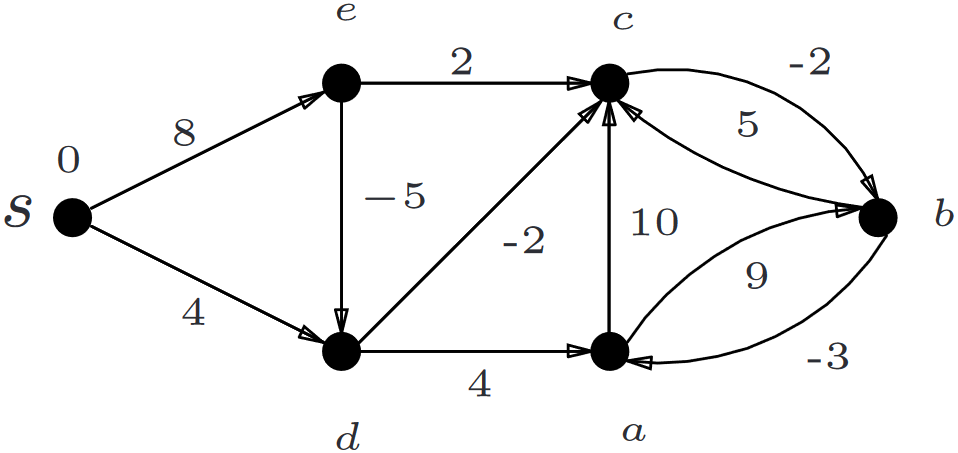
\includegraphics[clip,width=0.7\columnwidth]{Slike/341.png}
}

\subfloat[]{
  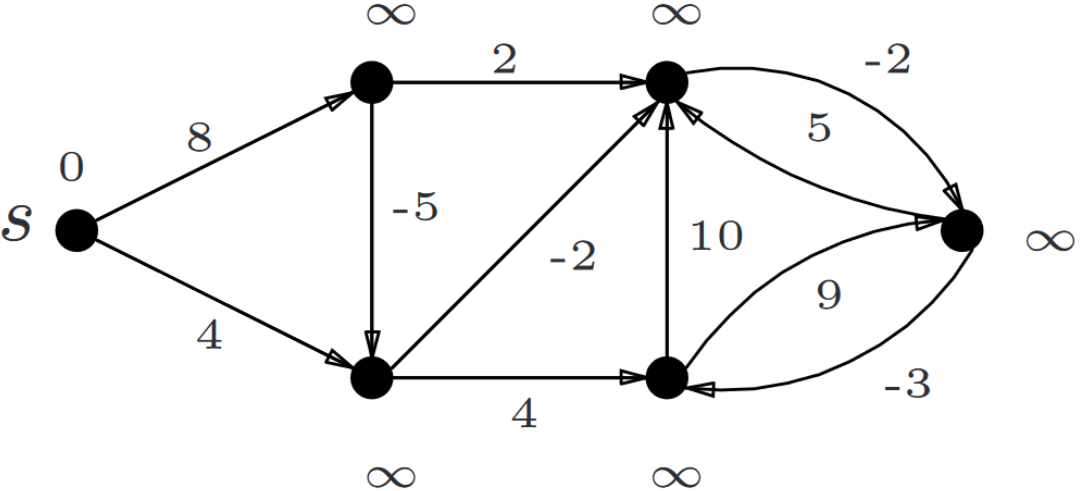
\includegraphics[clip,width=0.7\columnwidth]{Slike/34a.png}
}

\subfloat[]{
  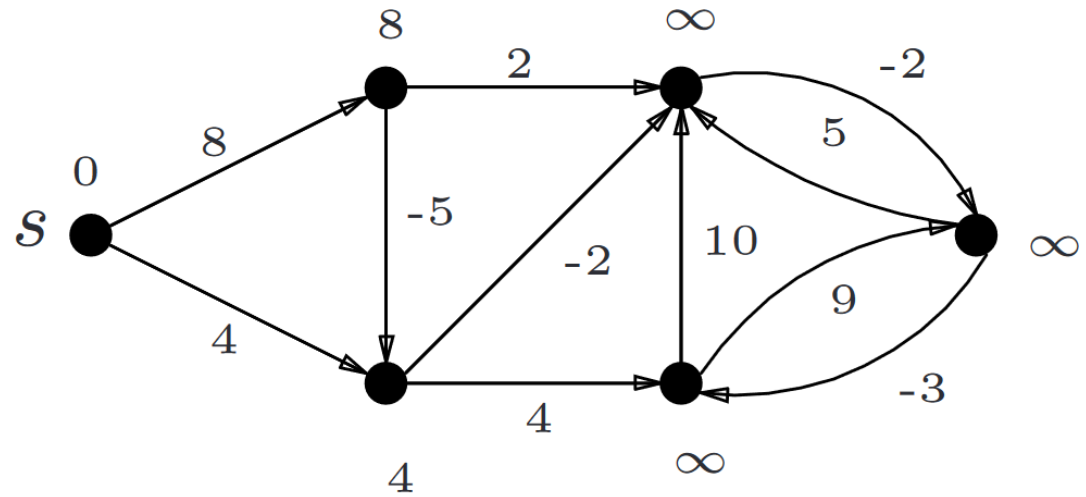
\includegraphics[clip,width=0.7\columnwidth]{Slike/34b.png}
}

\caption[]{Izvršavanje Bellman-Ford algoritma. Za unutarnju petlju drugog koraka algoritma grane su razmatrane po leksikografskom slijedu: $ab, ac, ba, bc, cb, da, dc, ec, ed, sd, se$. a) Ulazni graf sa označenim čvorovima i težinom grana. b) Zadate su početne vrijednosti parametra $\delta$ uz čvorove. Stanje nakon prvog koraka algoritma c) Stanje nakon prve iteracije drugog koraka algoritma\cite{bang2008digraphs}.}\label{fig:341}
\end{figure}

\begin{figure}[H]
    \centering
\subfloat[]{
  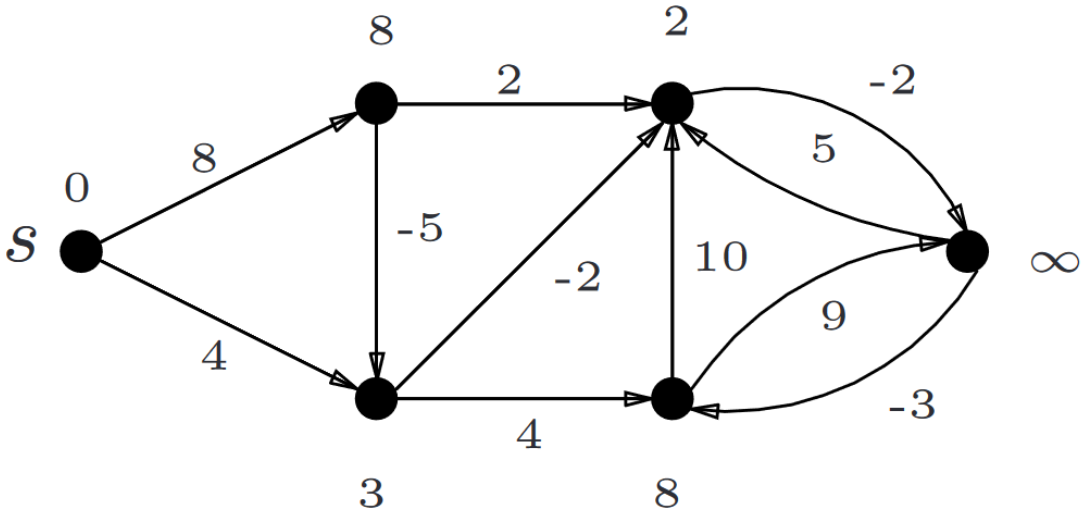
\includegraphics[clip,width=0.7\columnwidth]{Slike/34c.png}
}

\subfloat[]{
  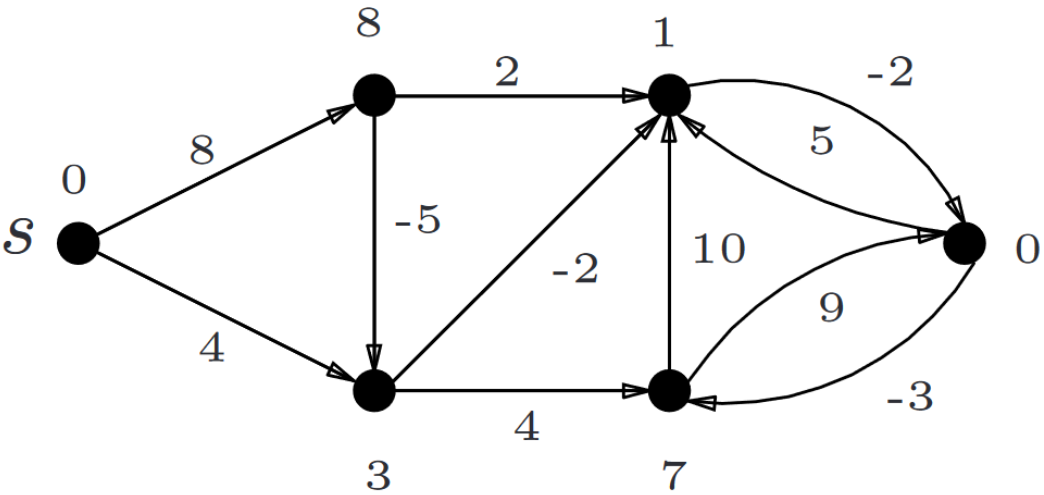
\includegraphics[clip,width=0.7\columnwidth]{Slike/34d.png}
}

\subfloat[]{
  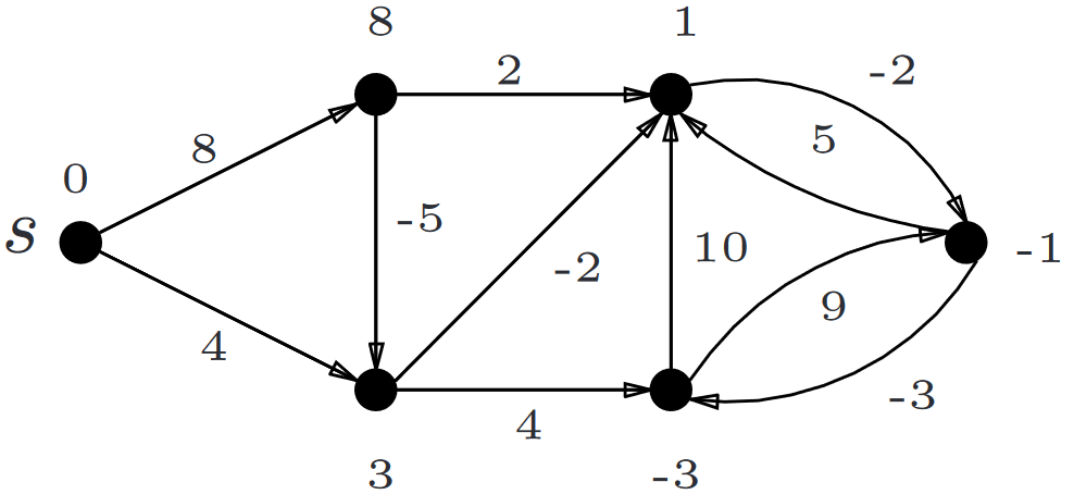
\includegraphics[clip,width=0.7\columnwidth]{Slike/34e.png}
}

\subfloat[]{
  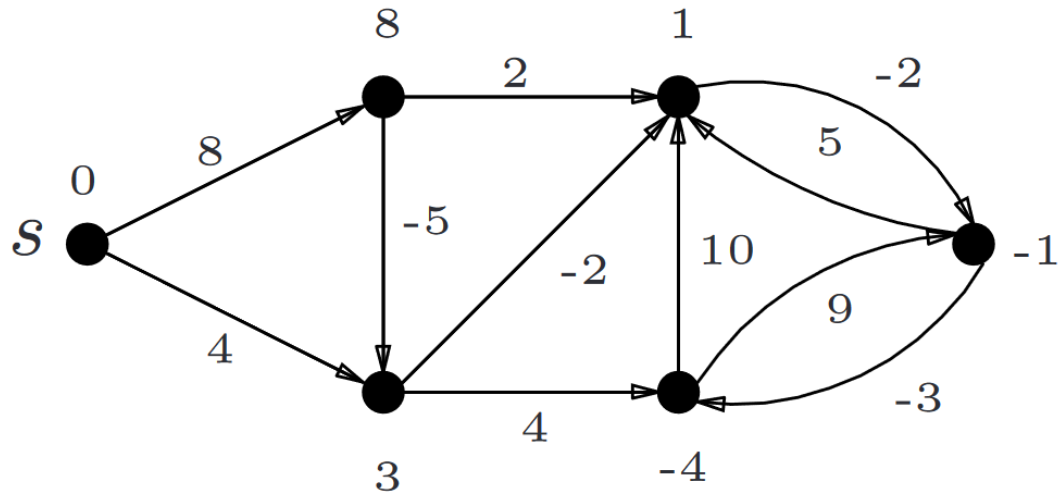
\includegraphics[clip,width=0.7\columnwidth]{Slike/34f.png}
}

\caption[]{(a) do (d) Stanja nakon svake uzastopne iteracije  unutarnje petlje drugog koraka algoritma do kraja\cite{bang2008digraphs}.}\label{fig:342}
\end{figure}









\section{Simulacijski rezultat}

Potpuna implementacija prethodno objašnjenog Bellman-Ford algoritma je data u prilogu ovog rada. U prilogu su isto tako date implementacije Dijkstrinog i Floyd-Warshallovog algoritma. U nastavku će biti objašnjeni glavni dijelovi sva tri algoritma kao i njihova usporedba. %Kako se ovaj rad fokusira na poređenje Bellman-Ford algoritma sa Dijkstrinim i Floyd-Warshallovim algoritmom, pokazane su i implementacije i ta dva algoritma pod Kod \ref{Kod_Dijkstra} i \ref{Kod_Floyd_Warshall} (svi kodovi i isječci u ovom radu koriste \lstinline{solarized light} temu \cite{solarized}). 


Komuptacijska kompleksnost algoritma predstavlja količinu vremena, memorije ili drugih resursa kako bi se algoritam izvršio. U ovom radu je korišten broj iteracija prilikom računanja najkraćeg puta kao parametar za računanje kompleksnosti navedena tri algoritma.

Za Bellman-Ford algoritam, komputacijska kompleksnost je $\mathcal{O}(n \cdot m)$ (u najgorem slučaju), dok za Dijkstrin algoritam je $\mathcal{O}(m + n \cdot \log{n})$ (u najgorem slučaju) i za Floyd-Warshallov algoritam je $\mathcal{O}(n^3)$ (ista je kompleksnost i za najbolji i za najgori slučaj). U prethodnim formulama $n$ predstavlja broj čvorova a $m$ predstavlja broj grana unutar grafa.

Neka je dat graf kao na slici \ref{sl:testni_graf} (postavka grafa je preuzeta sa \cite{juric_pomocno}, dok je slika grafa je preuzeta sa \cite{visualgo}). Potrebno je pronaći najkraći put od 0-tog do 11-tog čvora.

\begin{figure}[H]
    \centering
    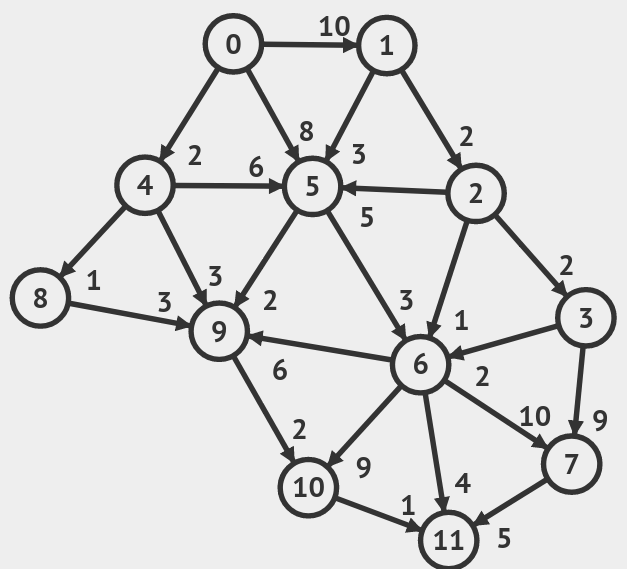
\includegraphics[scale=0.3]{Slike/primjer_grafa.png}
    \caption{Testni graf}
    \label{sl:testni_graf}
\end{figure}

Svi algoritmi koriste .txt datoteku u kojoj je opisan graf kako bi generisali traženi minimalni put od početnog do krajnjeg čvora. Datoteka \textit{upis.txt}, data u prilogu ovog rada, koja se koristi u svim kodovima sadrži opis grafa sa slike \ref{sl:testni_graf}. Prve dvije linije predstavljaju broj čvorova i broj grana, nakon toga linije opisuju cijenu puteva od susjednih čvorova i kako su usmjereni, a zadnje dvije linije datoteke sadrže broj početnog i krajnjeg čvora (u ovom primjeru 0-ti i 11-ti čvor). U svim kodovima zamjenom \lstinline{fin} sa \lstinline{std::cin} i \lstinline{fout} sa \lstinline{std::cout} će se preći sa datotečnog upisa-ispisa na konzolni upis-ispis.

Datoteka se učitava kroz kod preko \lstinline{std::ifstream} toka iz \lstinline{<fstream>} biblioteke, a rezultat se upisuje u novu .txt datoteku preko \lstinline{std::ofstream} toka iz istoimene bibilioteke.

Glavni dio implementacije Bellman-Ford algoritma je dat u nastavku pod Kod \ref{Kod_Bellman} (svi kodovi unutar rada koriste temu \lstinline{solarized light}\cite{solarized}), prije čega se inicijaliziraju potrebne vrijednosti za broj čvorova i broj grana, kao što se i unesu vrijednosti cijena puteva unutar grafa (što se uradi preko tokova kako je opisano u prethodnom pasusu).

Kao što se može vidjeti, prvo se inicijaliziraju cijene svih grana (\lstinline{std::vector<int> distance} u kodu) na $\infty$ tj. na $2^{29}$ zbog toga što ako se dvije takve putanje saberu, onda se ne prekorači maksimalna vrijednost \lstinline{int} tipa u C++ programskom jeziku koja iznosi $2^{31} - 1$. Vrijednost $2^{29}$ je svakako veća od bilo koje putanje unutar grafa, što simbolički označava $\infty$. Za početni čvor stavimo da je udaljen za cijenu 0 od samog sebe.

Ukoliko možemo prolaskom kroz čvor sa indeksom \lstinline{ivice.at(j).first} (\lstinline{std::vector<std::pair<int, int> > ivice} inicijaliziran prije glavnog dijela algoritma kroz datoteku \textit{upis.txt}) i ivicu sa indeksom \lstinline{j} (na isti način inicijaliziran vektor \lstinline{std::vector<int> tezine_ivica} smanjiti udaljenost čvora sa indeksom \lstinline{ivice.at(j).second} od početnog čvora, to se i uradi.

Varijabla \lstinline{flag} koja je \textit{boolean} tipa služi kako bi algoritam završio sa izvršavanjem čim je izvjesno da su pronađene najkraće putanje od početnog čvora.

Druga varijabla \textit{boolean} tipa, varijabla u kodu \lstinline{flag_neg_ciklusi}, služi za detekciju negativnih ciklusa - ukoliko nakon pronalaska najkraćih puteva prolaskom kroz sve ivice neka od udaljenosti čvorova od početnog čvora se ažurira, onda po Teoremu \ref{th:neg_ciklus} graf sadrži negativan ciklus i ne postoje najkraće putanje od početnog čvora ka svim ostalim čvorovima u grafu.

\begin{lstlisting}[language=C++, caption=Implementirani kod za Bellman-Ford algoritamm, label={Kod_Bellman}]
    // Za svaki cvor se pamtni koliko je udaljen od pocetnog cvora
    // Inicijalizirani su na 2^29 (beskonacno za nase svrhe)
    std::vector<int> distance(br_cvorova, 1 << 29);
    // Za pocetni cvor znamo da nije beskonacno udaljen od samog sebe:
    distance.at(pocetni_cvor) = 0;

    int broj_iteracija = 0;
    for(int i = 0; i < br_cvorova - 1; i++) {
        bool flag = false;
        for(int j = 0; j < br_ivica; j++) {
            if(distance.at(ivice.at(j).first) + tezine_ivica.at(j) <  distance.at(ivice.at(j).second)) {
                distance.at( ivice.at(j).second ) = distance.at( ivice.at(j).first ) + tezine_ivica.at(j);
                flag = true;
            }
            broj_iteracija++;
        }
        if(!flag) break;
    }

    bool flag_neg_ciklusi = false;
    for(int j = 0; j < br_ivica; j++) {
        if(distance.at(ivice.at(j).first) + tezine_ivica.at(j) <  distance.at(ivice.at(j).second)) {
            flag_neg_ciklusi = true;
        }
        broj_iteracija++;
    }

\end{lstlisting}

U nastavku je prikazana izlazna .txt datoteka za izvršeni Bellman-Ford algoritam nad navedenim primjerom pod Kod \ref{rezultat_Bellman}. 

\lstset{keywordstyle=\color{solarized-violet}}

\begin{lstlisting}[caption=Rezultat ispisa za Bellman-Fordov algoritma, label={rezultat_Bellman}]
***********************************
Najkraca distanca od 0-og do 11-og cvora iznosi: 8.
U grafu nema negativnih ciklusa.

Kompleksnost Bellman-Ford algoritma je O(broj cvorova * broj ivica) u najgorem slucaju.
Izracunate su najkrace udaljenosti od pocetnog do svakog drugog cvora.

Broj iteracija algoritma je bio 69 (jedna iteracija je poredjenje dvije vrijednosti duzina).
***********************************
\end{lstlisting}

\lstset{keywordstyle=\color{solarized-blue}\bfseries}

Glavni dio implementacije Dijkstrinog algoritma je dat u nastavku pod Kod \ref{Kod_Dijkstra}. Prije svega, za razliku od ostalih algoritama koji su prikazani u ovom radu, implementacija Dijkstrinog algoritma uključuje napredniju strukturu podataka koja se zove \lstinline{std::priority_queue}. \lstinline{std::priority_queue} omogućuje brz pristup najvećem elementu koji se nalazi u njemu. Također podržava brzo ubacivanje elemenata i brzo izbacivanje najvećeg elementa (sve sa $\mathcal{O}(\log{n})$ kompleksnosti).

Kako nam je potreban pristup najmanjem elementu, onda je potrebno modificirati \lstinline{std::priority_queue} tako da umjesto brzog prisupa najvećem elementu, imamo brz pristup najmanjem elementu. To se radi sljedećom konstrukcijom \lstinline{std::priority_queue<std::pair<int, int>, std::vector<std::pair<int, int> >, std::greater<std::pair<int, int> > >}, u slučaju da su elementi \lstinline{std::priority_queue}-a tipa \lstinline{std::pair<int, int>}, što je i implementirano unutar koda. Pri poređenju dvije varijable tipa \lstinline{std::pair<int, int>}, prvo se upoređuju prvi elementi parova, pa onda drugi.

Sa takvim tipom elementa onda se \lstinline{std::priority_queue} inicijalizira sa početnim čvorom i njegovom udaljenosti od samog sebe koja iznosi 0. Ovo se vrši komandom \lstinline{iduci_cvor.push(std::make_pair(0, pocetni_cvor))}. Primijetimo da je prvi element težina, a drugi element indeks čvora. Ovo je urađeno kako bi \lstinline{std::priority_queue} držao čvorove u željenom poretku.

Sada se ponavlja idući postupak unutar koda: posmatrajući čvor koji je najbliži početnom iz \lstinline{std::priority_queue}-a, svi njegovi susjedi koji nisu do sada posmatrani se dodaju u \lstinline{std::priority_queue} sa težinom jednakom zbiru težine trenutnog posmatranog čvora i težine veze između njih. To se postiže linijom \lstinline{iduci_cvor.push( std::make_pair( trenutni_cvor.first + x.second, x.first ) )}. 

Prvim posmatranjem konačnog čvora poznata je dužina optimalnog puta do njega. Ova činjenica nije iskorištena za optimizaciju koda ispod. Umjesto toga, korišten je jednostavniji kriterij zaustavljanja - ispražnjenje \lstinline{std::priority_queue}-a.

\begin{lstlisting}[language=C++, caption=Implementirani kod za Dijkstrin algoritam, label={Kod_Dijkstra}]
    // Pravimo priority queue da bismo znali koji je preostali cvor najblizi pocetnom
    // Ovako ide konstrukcija ako zelimo da priority queue daje prednost najmanjem, a ne najvecem
    std::priority_queue<std::pair<int, int>, std::vector<std::pair<int, int> >, std::greater<std::pair<int, int> > > iduci_cvor;
    std::vector<bool> posjecen(br_cvorova, false);

    // Pocetni cvor je uvijek 0 udaljen od samog sebe:
    iduci_cvor.push(std::make_pair(0, pocetni_cvor));
    int udaljenost = -1;

    int broj_iteracija = 0;
    std::pair<int, int> trenutni_cvor;
    while(!iduci_cvor.empty()) {
        trenutni_cvor = iduci_cvor.top();
        iduci_cvor.pop();
        if(posjecen.at(trenutni_cvor.second)) continue;
        posjecen.at(trenutni_cvor.second) = true;
        if(trenutni_cvor.second == krajnji_cvor) {
            udaljenost = trenutni_cvor.first;
        }
        // Moramo proci kroz sve susjede od trenutni_cvor.first
        for(auto x : susjedstva.at(trenutni_cvor.second)) {
            if(posjecen.at(x.first)) continue;
            iduci_cvor.push( std::make_pair( trenutni_cvor.first + x.second, x.first ) );
            broj_iteracija++;
        }
    }
}
\end{lstlisting}

U nastavku je prikazana izlazna .txt datoteka za izvršeni Dijkstrin algoritam nad navedenim primjerom pod Kod \ref{rezultat_Dijkstra}. 

\lstset{keywordstyle=\color{solarized-violet}}

\begin{lstlisting}[caption=Rezultat ispisa za Dijkstrin algoritam, label={rezultat_Dijkstra}]
***********************************
Najkraca distanca od 0-og do 11-og cvora iznosi: 8.

Kompleksnost Dijkstra algoritma je O(broj ivica + broj cvorova * log(broj cvorova)) u najgorem slucaju.
Izracunata je samo potrebna distanca.

Broj iteracija algoritma je bio 14 (jedna iteracija je poredjenje dvije vrijednosti duzina).
***********************************
\end{lstlisting}


\lstset{keywordstyle=\color{solarized-blue}\bfseries}

Glavni dio Floyd-Warshallovog algoritma je dat pod Kod \ref{Kod_Floyd_Warshall}. Ovaj algoritam koristi tzv. matricu susjedstva kako bi se držale procjene udaljenosti između svaka dva čvora u grafu. Ovaj algoritam radi na sljedeći način: posmatraju se sve trojke čvorova grafa ($A, \; B, \; C$). Ukoliko je zbir udaljenosti od $A$ do $B$ i od $B$ do $C$ manji od trenutne procijenjene udaljenosti od $A$ do $C$, onda se ažurira udaljenost od $A$ do $C$.

Na početku su sve međusobne udaljenosti postavljene na $\infty$, osim udaljenosti čvorova od samih sebe i od čvorova sa kojima imaju neposrednu vezu putem jedne od grana grafa. 

\begin{lstlisting}[caption=Implementirani kod za Floyd-Warshallov algoritam, label={Kod_Floyd_Warshall}]
    int broj_iteracija = 0;
    for(int i = 0; i < br_cvorova; i++) {
        for(int j = 0; j < br_cvorova; j++) {
            for(int k = 0; k < br_cvorova; k++) {
                if(matrica_udaljenosti.at(i ).at(j) + matrica_udaljenosti.at(j ).at(k) < matrica_udaljenosti.at( i ).at(k))
                    matrica_udaljenosti.at(i ).at(k) = matrica_udaljenosti.at( i).at(j) + matrica_udaljenosti.at( j).at(k);
                broj_iteracija++;
            }
        }
    }
\end{lstlisting}

U nastavku je prikazana izlazna .txt datoteka za izvršeni Floyd-Warshallov algoritam nad navedenim primjerom pod Kod \ref{rezultat_Floyd}. 

\lstset{keywordstyle=\color{solarized-violet}}

\begin{lstlisting}[caption=Rezultat ispisa za Dijkstrin algoritam, label={rezultat_Floyd}]
***********************************
Najkraca distanca od 0-og do 11-og cvora iznosi: 8.

Kompleksnost Floyd-Marshall algoritma je O((broj cvorova)^3) u najgorem slucaju.
Izracunate su najkrace udaljenosti od svakog pocetnog do svakog drugog cvora.

Broj iteracija algoritma je bio 1728 (jedna iteracija je poredjenje dvije vrijednosti duzina).
***********************************
\end{lstlisting}

Kao što se može vidjeti, Dijkstrin algoritam je u najmanje iteracija došao do rezultata za 14 iteracija, Bellman-Fordov algoritam je za 69 iteracija došao do rezultata, dok je Floyd-Warshallov algoritam došao do rezultata za 1728 iteracija.

Dobiveni rezultat je očekivan zbog toga što Dijkstrin algoritam računa samo potrebnu distancu (tj. samo distancu od 0-tog do 11-tog čvora), Bellman-Ford algoritam računa najkraće udaljenosti od početnog, 0-tog čvora u ovom slučaju, do svakog drugog čvora unutar grafa, dok Floyd-Warshallov algoritam je izračunao sve najkraće udaljenosti od bilo kojeg čvora do drugog bilo kojeg čvora u grafu.

Na slikama \ref{sl:graf1}, \ref{sl:graf2}, \ref{sl:graf3} i \ref{sl:graf4} je prikazana usporedba procijenjenog broja iteracija svakog od ova tri algoritma. Procjene su napravljene direktno preko formula iz kompleksnosti ovih algoritama.

Ukoliko je broj čvorova $n$, onda je uzeta aproksimacija da je broj grana jednak $n \cdot \sqrt{n}$ (ovo je uzeto kao procjena grafa koji nije ni naročito gust ni naročito rijedak).

Sa grafika se jasno može vidjeti da je Dijkstrin algoritam najbrži, dok je Floyd-Warshall algoritam najsporiji. Bellman-Ford algoritam nudi dobar kompromis između brzine izvršavanja i opsega primjenjivosti. Također, on je jedini od ova tri algoritma koji je pogodan za primjenu nad distribuiranim sistemima.

\begin{figure}
    \centering
    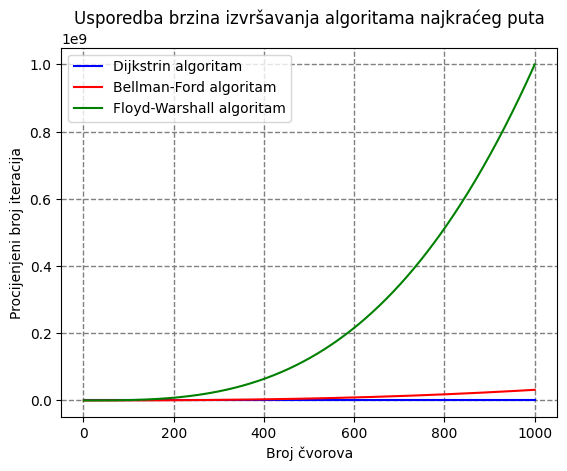
\includegraphics[width=8cm]{Slike/graf1.png}
    \caption{Usporedba brzina izvršvanja Dijkstrinog, Bellman-Ford i Floyd-Warshall algoritma za broj čvorova do 1000}
    \label{sl:graf1}
\end{figure}

\begin{figure}
    \centering
    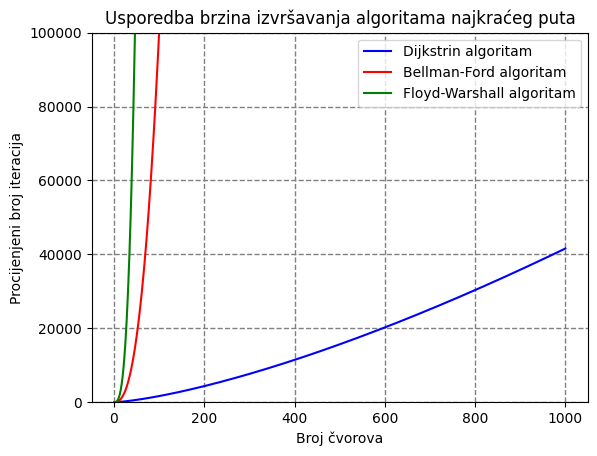
\includegraphics[width=8cm]{Slike/graf2.png}
    \caption{Usporedba brzina izvršvanja Dijkstrinog, Bellman-Ford i Floyd-Warshall algoritma za broj čvorova do 1000, ali je grafik uvećan}
    \label{sl:graf2}
\end{figure}

\begin{figure}
    \centering
    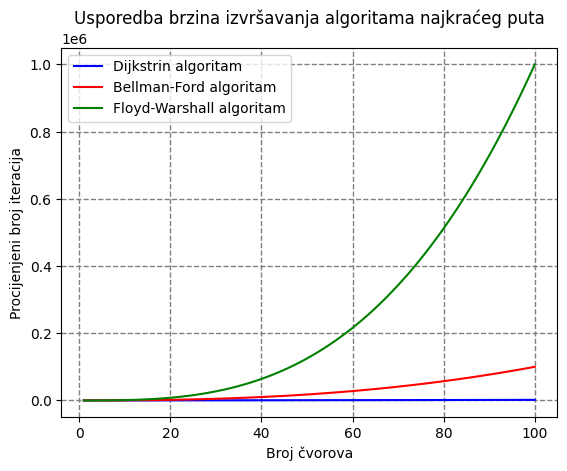
\includegraphics[width=8cm]{Slike/graf3.png}
    \caption{Usporedba brzina izvršvanja Dijkstrinog, Bellman-Ford i Floyd-Warshall algoritma za broj čvorova do 100}
    \label{sl:graf3}
\end{figure}

\begin{figure}
    \centering
    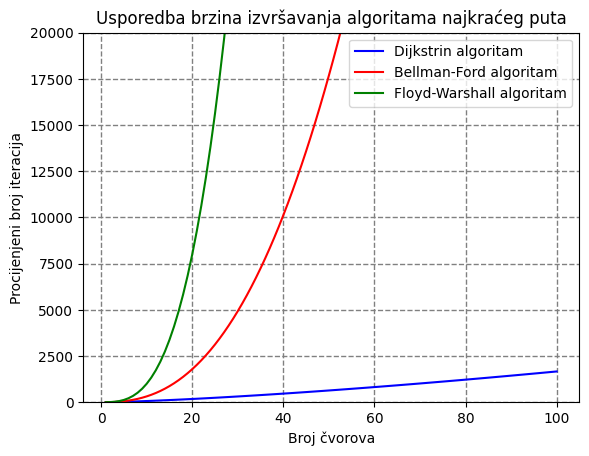
\includegraphics[width=8cm]{Slike/graf4.png}
    \caption{Usporedba brzina izvršvanja Dijkstrinog, Bellman-Ford i Floyd-Warshall algoritma za broj čvorova do 100, ali je grafik uvećan}
    \label{sl:graf4}
\end{figure}



\section*{Zaključak}
U radu je opisan problem pronalaska najkraćeg puta u usmjerenim težinskim grafovima. Za rješenje ovog problema predloženi su Dijsktrin algoritam kao i Floyd-Warshallov algoritam. Međutim uočeno je da ovi algoritmi imaju određena ograničenja kada su u pitanju grafovi sa negativnim težinama ili kada grafovi sadrže negativne cikluse. Iz tog razloga ovaj rad se fokusirao na Bellman-Fordov algoritam koji se može primijeniti upravo na takve grafove. Najprije je dat matematski opis i dokaz algoritma kao i pseudokod algoritma, a zatim implementacija u proramskom jeziku C++. U svrhu poređenja Bellman-Fordovog algoritma također su razvijene implementacije Dijsktrinog algoritma kao i Floyd-Warshallov algoritma.  C++ je korišten sa ciljem pouzdanijeg vremena izvršavanja (pošto je kompajlirani jezik i nema \textit{garbage collector}-a). No, kako su grafovi koji su korišteni mali, vrijeme izvršavanja se nije moglo precizno odrediti, tako da smo uporedili broj iteracija pri izvršavanju svakog od algoritama, te su prokomentarisani očekivani rezultati.

Kako bi se maksimizirala iskoristivost svakog od ovih algoritama, potrebno ih je koristiti u odgovarajućim kontekstima, dakle ako je potrebno da se nađe samo najkraća udaljenost od nekog početnog čvora do nekog drugog krajnjeg čvora u grafu bez negativnih grana, onda bi tu Dijkstrin algoritam bio najpogodniji, dok bi Floyd-Warshallov algoritam tu bio suvišan.

Bitno je naglasiti da iako je Dijkstrin algoritam najbrži, ipak Bellman-Ford algoritam može detektovati negativne cikluse, dok Dijkstrin algoritam ne može raditi u grafovima sa negativnim težinama granama. Floyd-Warshall algoritam može detektovati i negativne cikluse, ali nije pogodan za to jer se onda mora modificirati.
\printbibliography
\end{document}
